\chapter{Introduction\label{chap:intro}}

% What are optimization problems and where do they occur
% Start by telling a story (running example throughout intro)
Optimization problems can be summarized as the task of finding a ``best'' solution out of a collection of feasible ones.
For example, when looking for a new flat to buy, most people will be comparing prices with the aim to find the cheapest flat possible that fulfils their requirements.
Commonly, the notion of ``best'' that is used in optimization is that a solution with minimum associated ``cost'' is considered optimal.
Speaking in the example from above, this cost is the price of the flat.
If the collection of possible solutions is discrete (as in this example), we speak of \emph{combinatorial} optimization.

% Reveal conflicting second objective
Looking more closely at the flat search example, we can notice a problem emerging:
what does ``fulfilling'' the requirements mean?
Some requirements, like the number of rooms, might be easy to specify, but consider the distance of ones daily commute.
Rather than setting a fixed threshold as ``maximum $d$ kilometres distance'', what we might actually want to do is minimize this distance at the same time as the cost of the flat.
Now there are two objectives to take into account regarding what constitutes a ``best'' solution.
Two objectives give rise to \emph{bi-objective} optimization, which we study in this work.

% Approaches to solving optimization
Since combinatorial optimization is relevant for real-world problems, a plethora of algorithmic approaches to solving optimization problems have been proposed.
These approaches range from local search~\autocite{DBLP:books/daglib/0017492}, over evolutionary~\autocites{DBLP:books/daglib/0087893,DBLP:journals/jgo/StornP97} to declarative programming-based algorithms~\autocite{handbook2-maxsat,ChenEtAl2010-intro,DBLP:reference/fai/2}.
In addition to these generally applicable approaches, there are problem specific algorithms (e.g.,~\autocite{DBLP:conf/aaai/DemirovicS21,DBLP:conf/kdd/NijssenF07,DBLP:conf/nips/HuRS19}).
One other attribute on which the optimization approaches differ is whether they are exact or approximative.
Given enough resources, an exact algorithm is guaranteed to find \emph{the best} solution, while approximative algorithms will return \emph{a good} solution within given resource constraints.

% MaxSAT (and SAT)
In this work, we present a declarative programming approach for finding exact Pareto-optimal solutions to bi-objective optimization problems.
We use propositional logic as the declarative programming language and build on maximum satisfiability (MaxSAT) solving techniques.
MaxSAT is the \NP-hard single-objective optimization variant of the \NP-complete propositional satisfiability (SAT) problem.
It asks for an assignment to a given propositional formula, maximizing the number of satisfied clauses.
Solvers for MaxSAT have made significant progress over the recent years and are by now very efficient for solving many practical optimization problems.
This progress is mainly due to development on the underlying SAT solvers used in MaxSAT solving~\autocites{DBLP:journals/ai/FroleyksHIJS21,handbook2-cdcl}, but also due to improved algorithms for how to apply those SAT solvers in MaxSAT solving.
Some approaches for SAT- and MaxSAT-based bi--objective optimization have been proposed in the past~\autocites{DBLP:conf/cp/SohBTB17,DBLP:conf/ijcai/Terra-NevesLM18a,DBLP:conf/aaai/Terra-NevesLM18,DBLP:conf/ijcai/Terra-NevesLM18,DBLP:conf/cp/JanotaMSM21}, but it is not a very active field of research.
We seek to extend the progress and success in MaxSAT solving to two objectives.

% Hardness of optimization problems
Combinatorial optimization problems are typically hard to solve.
We informally extend the complexity class \NP{}~\autocite{AroraBarak2009-complexity} to optimization problems.
While $\mathcal{P}$ contains all decision problems for which an algorithm that solves the problem in polynomial time is known, such an algorithm is not known for problems that are in \NP{} but not $\mathcal{P}$.
This means that the worst case runtime for \NP-complete (i.e., exactly as hard as the hardest problems in \NP) and \NP-hard (i.e., at least as hard as problems in \NP) problems is exponential.
Informally, we say an optimization problem is \NP-hard if its corresponding decision problem is \NP-complete.
Consider the \NP-complete set covering decision problem~\autocite{DBLP:conf/coco/Karp72} where for a collection $\sets$ of sets, the task is to determine whether a cover $\cover$ with cardinality smaller than a threshold $k$ exists so that the cover intersects all sets, i.e., $S \cap \cover \neq \emptyset$ for all $S\in\sets$.
The corresponding optimization problem, where the task is to find the \emph{smallest} such cover is \NP-hard.
Several other well known \NP-complete decision problems also have corresponding \NP-hard optimization problems~\autocite{KorteVygen2018-15}.

% Applications of (single- and bi-objective) optimization in literature
\NP-hard single- and bi-objective optimization problems arise naturally in many areas, ranging from industrial applications over research to everyday tasks.
While the single-objective case has been studied in depth for tasks including scheduling~\autocites{DBLP:conf/cp/Stojadinovic14,DBLP:conf/cpaior/BofillGSV15,DBLP:journals/ior/Solomon87,DBLP:journals/candie/AkyolB07}, supply chain optimization~\autocite{DBLP:journals/cce/Papageorgiou09}, air traffic management~\autocites{DBLP:journals/ior/BertsimasLO11,RichardsHow2002Aircrafttrajectoryplanning}, clustering~\autocite{DBLP:journals/ai/DaoDV17,DBLP:conf/sdm/DavidsonRS10} and learning optimal classifiers~\autocites{DBLP:conf/cp/MaliotovM18,DBLP:conf/ijcai/NarodytskaIPM18,DBLP:conf/ijcai/Hu0HH20,DBLP:conf/cp/YuISB20,DBLP:conf/aaai/DemirovicS21,DBLP:conf/cp/ShatiCM21,DBLP:conf/cade/IgnatievPNM18}, the bi-objective setting has not been studied as much.
Some of the fewer examples from literature are the following:
When learning interpretable classifiers~\autocites{DBLP:conf/ijcai/Ignatiev0NS21,DBLP:conf/cp/MaliotovM18,DBLP:conf/ijcai/NarodytskaIPM18,DBLP:conf/ijcai/Hu0HH20,DBLP:conf/cp/YuISB20,DBLP:conf/aaai/Ignatiev0S021,DBLP:conf/cade/IgnatievPNM18}, the objectives ``interpretability'' and ``classification error'' are in conflict because a more complex and therefore less interpretable classifier is typically more accurate.
A bi-objective optimization problem arises when wanting to create a portfolio of solvers that together solve a set of benchmarks as fast as possible while also containing as few solvers as possible~\autocite{DBLP:conf/cp/JanotaMSM21}.
There are also bi-objective optimization problems in network routing with the objectives load balancing and latency~\autocite{SilverioEtAl2022biobjectiveoptimization}.
In supply chain optimization, in addition to the economic objective, environmental aspects can be taken into consideration as a second objective~\autocites{DBLP:journals/cce/Pinto-VarelaBN11,DBLP:journals/candie/TautenhainBN19}.

% Solving pipeline for declarative approaches
The declarative programming approach, that is generally applicable to all of these applications, follows the solving pipeline illustrated in \cref{fig:solving-pipeline}.
First, the problem of interest is \emph{encoded} into a set of constraints formulated in a declarative programming language of choice.
Examples of declarative languages for optimization are MaxSAT~\autocite{handbook2-maxsat}, constraint programming~\autocite{DBLP:reference/fai/2} and mixed integer linear programming~\autocites{ChenEtAl2010-intro,KorteVygen2018-5}.
An encoding is hereby a mapping of each instance of the original problem to a set of constraints in the declarative language, where each optimal solution to the encoded instance corresponds to an optimal solution to the original instance.
Choosing a fitting declarative language for solving a given problem is a non-trivial problem and doing so should take considerations such as how succinctly a language can represent a problem into account.
Secondly, a general optimization solver for the declarative language is used to solve the encoded problem and obtain on optimal solution for it.
A solver for a declarative programming language is an algorithm that finds an optimal solution to an instance in said language.
The last step is to map the found solution back to the original problem space.

\begin{figure}
  \centering
  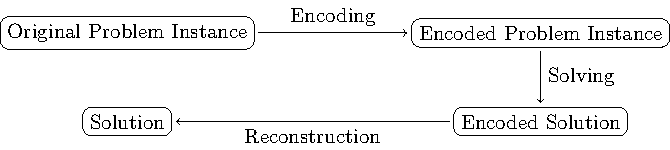
\includegraphics{solving-pipeline.pdf}
  \caption{The solving pipeline of the declarative approach to optimization.}\label{fig:solving-pipeline}
\end{figure}

% Advantages of declarative approaches
When solving an optimization problem with the declarative approach, the task that needs to be solved is \emph{not} coming up with a new algorithm but only with an encoding of the problem into constraints in the used language.
However, this general applicability is not the only advantage.
Improvement in solver performance for a declarative language also immediately maps to better solving performance for \emph{all} problems that can be encoded in said language.

% Runtimes in declarative approaches
In the scope of this work, we focus on using the declarative approach for solving \NP-hard optimization problems.
For this application, \NP-hard declarative languages are used.
Given an existing encoding for the problem, this means that the generic solving step is the only computationally hard step in the solving pipeline.
Both the encoding and the reconstruction of the solution are typically done in polynomial time.
Since the declarative language is \NP-hard, the worst-case runtime of the solving algorithm cannot be better than exponential (assuming $\mathcal{P}\neq\mathcal{NP}$).
However, in practice one can observe significantly better performance from many solving algorithms for ``interesting'' instances, i.e., instances that appear for real-world problems.
Exemplary solving algorithms for \NP-hard declarative languages that achieve good performance on real-world instances are MaxSAT solving algorithms~\autocite{handbook2-maxsat} based on conflict driven clause learning solvers for propositional satisfiability~\autocite{handbook2-cdcl}, and state-of-the-art branch-and-cut algorithms for mixed integer linear programming~\autocite{ChenEtAl2010-branch-and-cut}.

% Conflicting objectives and why there might be no single optimal solution
A crucial difference between single-objective and bi-objective optimization is that there is no single notion of optimality for two or more objectives.
Whereas for a single objective function, there is a clear minimum (or maximum) and objective values can be unambiguously compared, this becomes less defined for the bi-objective case:
coming back to the flat search example, consider a flat with a cost of 300\,000 \texteuro{} and 1-kilometre daily commute and compare it to another flat that costs 240\,000 \texteuro{} and has a 3-kilometre daily commute.
It is not immediately clear which one of these options is better, and the choice would depend on ones personal preference over the two objectives.
This becomes especially difficult if there is no clear preference over the objectives.
Typically, a situation like that occurs when two of the objectives considered are in conflict, as the price of a flat and the corresponding daily commute might be if the commute is towards the city centre and flats in the city centre are more expensive.

% Pareto optimality
% Point out different nomenclature
In the context of our work, the notion of optimality for bi-objective optimization is that of \emph{Pareto optimality} (also called \emph{efficiency} in other contexts)~\autocite{Ehrgott2005-2}.
Intuitively, under Pareto optimality a solution is considered optimal if no solutions that improve some objective without worsening the other exist.
This definition considers the two flats from earlier both equally optimal.
Under Pareto optimality, the task of solving a bi-objective optimization problem can mean multiple things:
finding a single Pareto-optimal solution, finding a representative solution for each Pareto point (also called non-dominated point in literature~\autocite{Ehrgott2005-2}), or finding all Pareto-optimal solutions.
Most approaches~\autocite{DBLP:conf/cp/SohBTB17,DBLP:conf/cp/JanotaMSM21,DBLP:conf/ijcai/Terra-NevesLM18a} to solving multi-objective optimization under Pareto optimality seem to focus on the second approach where a single solution per Pareto point (i.e., tuple of Pareto-optimal objective values) is computed.
The last task goes one step further and enumerates the full Pareto front (i.e., all Pareto-optimal solutions), even if multiple of the solutions might lead to the same objective values.
All three of these tasks can be solved by the algorithmic approach presented in this thesis.

% Bi-objective vs multi-objective
% Why bi-objective is interesting/enough
Going beyond the bi-objective setting, multi-objective optimization studies optimization problems with an arbitrary number of objectives.
The handle on multiple objectives and what the objective values of an optimal solution actually mean can quickly become hard to grasp.
As humans, we can only visualize three dimensions, meaning a Pareto front over four objectives is already an entirely abstract object while even a three-dimensional one is hard to visualize.
Two objectives, however, form a good trade-off between gaining meaningful information from the second objective over just using a single one, being able to intuitively visualize the Pareto front and not resulting in too many Pareto-optimal solutions.
Additionally, objectives that are considered ``less important'' but should still somehow be included in the optimization can still be added as a threshold constraint.

% Contributions
% Algorithm: single SAT solver; builds on MaxSAT; single vs all
The main contribution of this work is the \algname{} algorithm, a MaxSAT-based bi-objective optimization approach.
\algname{} builds on advances in MaxSAT solving, allowing for variants based on different solution-improving~\autocites{handbook2-maxsat,DBLP:journals/jsat/BerreP10,DBLP:journals/jsat/EenS06} and core-guided~\autocites{DBLP:journals/corr/abs-0712-1097,DBLP:conf/sat/AnsoteguiBL09,DBLP:conf/cp/MorgadoDM14,DBLP:journals/jsat/IgnatievMM19} algorithms.
We propose five different variants of \algname{}, the first four building on the SAT-UNSAT~\autocite{DBLP:journals/jsat/BerreP10}, UNSAT-SAT~\autocite{DBLP:conf/sat/FuM06}, MSU3~\autocite{DBLP:journals/corr/abs-0712-1097} and OLL~\autocite{DBLP:conf/cp/MorgadoDM14} MaxSAT algorithms.
The fifth variant is a hybrid between SAT-UNSAT search and MSU3, aiming to combine the advantages of the two approaches.
In addition to five variants of \algname{}, we also propose multiple refinements for improving its performance:
lazily building the cardinality constraints for both objectives, blocking dominated solutions, domain-specific blocking, bound hardening and other refinements known from core-guided MaxSAT solving.
\algname{} allows for solving all three tasks for bi-objective optimization:
finding a single Pareto-optimal solution, one representative solution for each Pareto point or enumerating all Pareto-optimal solutions.

% Evaluation: study efficiency of different MaxSAT algorithms
After proposing \algname{}, we empirically evaluate the performance of it on two benchmark domains:
learning interpretable decision rules from binary data~\autocite{DBLP:conf/cp/MaliotovM18} and bi-objective set covering.
In the experiments, we compare all five variants of \algname{} to three SAT-based competitors:
enumeration of $P$-minimal solutions~\autocite{DBLP:conf/cp/SohBTB17}, ParetoMCS enumeration~\autocite{DBLP:conf/ijcai/Terra-NevesLM18a} and Seesaw~\autocite{DBLP:conf/cp/JanotaMSM21}.
As a result of this evaluation, we determine which variant of \algname{} is the best-performing overall.
Furthermore, for the best-performing variant, we study the effects of the proposed refinements to determine their effectiveness.

% Signposting for chapters
This thesis is structured as follows:
An overview of propositional satisfiability and maximum satisfiability, highlighting the important preliminaries needed to understand the proposed algorithm, is given in \cref{chap:satisfiability}.
In \cref{chap:biobjective-optimization}, we introduce bi-objective optimization, defining the problem and surveying some existing approaches, based on SAT and other declarative paradigms, as well as probabilistic and meta-heuristic approaches.
After that, in \cref{chap:approach}, \algname{} including five variants and some refinements is proposed.
Finally, in \cref{chap:experiments} we outline the experiments and results, and conclude the thesis in \cref{chap:conclusion}.